\section{Механизмы, поддерживающие высокую готовность}

\underline{Определение: } Высокая доступность (High Availability, HA) - это характеристика технической системы, разработанная для избежания невыполненного обслуживания путём уменьшения или управления сбоями и минимизации времени плановых простоев (\autocite{WikiHA}). Доступность часто измеряется в <<Nines>> (девятки).

Высокая готовность для каждой конкретной системы зависит от цели, для которой предназначена эта система. Для некоторых компаний высокая готовность значит максимальное downtime за год в несколько минут. Для других HA может значит downtime несколько часов в месяц.
\begin{figure}[h]
    \centering
    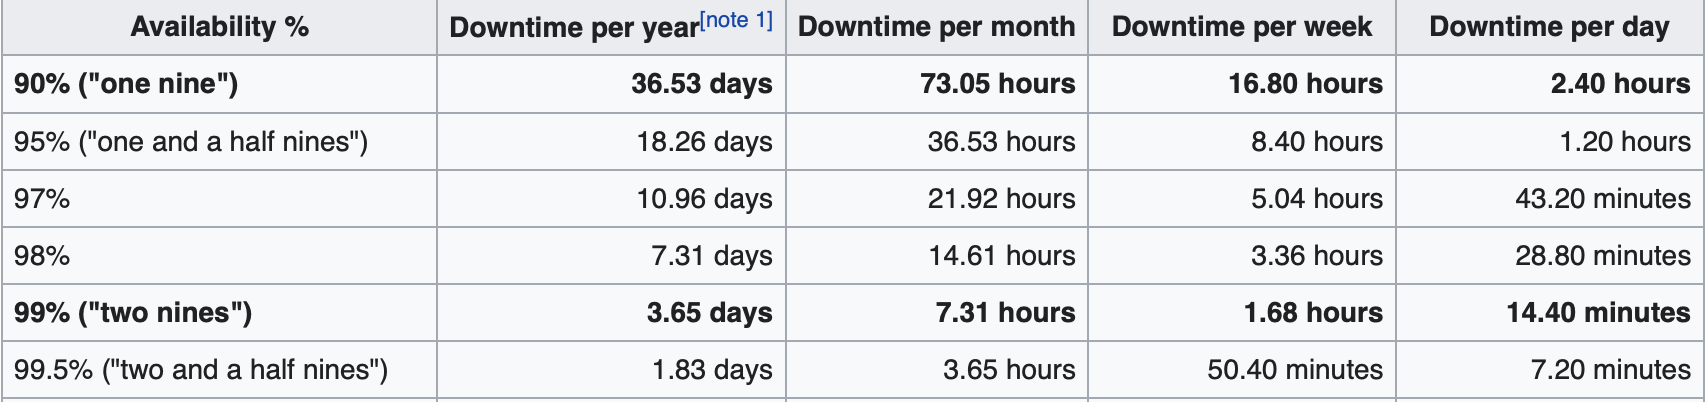
\includegraphics[width=0.8\textwidth]{assets/avail.png}
    \caption{Пример <<Nines>>}
    \label{fig:mesh1}
\end{figure}

HA включает в себя несколько важных аспектов:
\begin{enumerate}
    \item Доступность данных 
    \item Защита данных
    \item Производительность
    \item Цена поддержки
\end{enumerate}

\subsection{Средства, поддерживающие высокую готовность}
\paragraph{Аппаратная и программная поддержки}
Существует несколько возможных уровней обеспечения высокой готовности системы: аппаратный и программный уровни. \\
\underline{Аппаратный уровень} включает в себя:
\begin{enumerate}
    \item \underline{Репликация БД}
    Репликация позволяет скопировать данные с одного сервера бд на другой.
    Существуют  два подхода репликации баз данных, рассмотрим каждый из них (\autocite{Gregorchenko}):
    \begin{itemize}
        \item \underline{Репликация Master-Slave} \\В этом подходе выделяется один основной сервер базы данных, который называется Master. На нем происходят все изменения в данных (любые запросы INSERT/UPDATE/DELETE). Slave-сервер постоянно копирует все изменения с Master. С приложения на Slave-сервер могут отправляться запросы на чтение данных (запросы SELECT). Таким образом Master-сервер может отвечать за изменения данных, а Slave за чтение. Также Master сервер может отвечать за все операции с данными, а Slave являться бэкапом. При выходе из строя Slave, достаточно просто переключить все приложение на работу с Master. После этого восстановить репликацию на Slave и снова его запустить. Если выходит из строя Master, нужно переключить все операции (и чтения, и записи) на Slave. Таким образом он станет новым Master. После восстановления старого Master, настроить на нем реплику, и он станет новым Slave. Рассмотрена асинхронная репликация. При синхронной репликации результат сразу же записывается и в Master, и в Slave. Возвращение управления клиенту происходит только после записи в обе базы.
        \item \underline{Репликация Master-Master}\\ В этой схеме любой из серверов может использоваться как для чтения, так и для записи. При использовании такого типа репликации достаточно выбирать случайное соединение из доступных Master. Вероятные поломки делают Master-Master репликацию непрактичной. Выход из строя одного из серверов практически всегда приводит к потере каких-то данных. Последующее восстановление также сильно затрудняется необходимостью ручного анализа данных, которые успели, либо не успели скопироваться.
    \end{itemize}  

    Помимо разбиения репликаций по способу организации системы (см. выше) стоит выделить различные подходы по способу внесения изменений в базу данных. Рассмотрим на примере PostgreSQL, который поддерживает эти реализации(\autocite{PostrgreSQL1}).
    \begin{itemize}
        \item \underline{Потоковая репликация} \\Это репликация, при которой от основного сервера PostgreSQL на реплики передается WAL(журнал предзаписи транзакций). И каждая реплика затем по этому журналу изменяет свои данные. Для настройки такой репликации все серверы должны быть одной версии, работать на одной ОС и архитектуре. Потоковая репликация в Postgres бывает двух видов — асинхронная и синхронная.
		\begin{enumerate}
        		\item{Асинхронная репликация} \\В этом случае PostgreSQL сначала применит изменения на основном узле и только потом отправит записи из WAL на реплики. Преимущество такого способа — быстрое подтверждение транзакции, т.к. не нужно ждать пока все реплики применят изменения. Недостаток в том, что при падении основного сервера часть данных на репликах может потеряться, так как изменения не успели продублироваться.
        		\item{Синхронная репликация} \\В этом случае изменения сначала записываются в WAL хотя бы одной реплики и только после этого фиксируются на основном сервере. Преимущество — более надежный способ, при котором сложнее потерять данные. Недостаток — операции выполняются медленнее, потому что прежде чем подтвердить транзакцию, нужно сначала продублировать ее на реплике.
        	\end{enumerate}
        	\item \underline{Логическая репликация} \\Логическая репликация оперирует записями в таблицах PostgreSQL. Этим она отличается от потоковой репликации, которая оперирует физическим уровнем данных: биты, байты, и адреса блоков на диске. Возможность настройки логической репликации появилась в PostgreSQL 10.
Этот вид репликации построен на механизме публикации/подписки: один сервер публикует изменения, другой подписывается на них. При этом подписываться можно не на все изменения, а выборочно. Например, на Master-сервере 50 таблиц: 25 из них могут копироваться на один Slave-сервер, а 25 — на другой.
Также есть несколько ограничений, главное из которых — нельзя реплицировать изменения структуры БД. То есть если на Master-сервере добавится новая таблица или столбец — эти изменения не попадут в Slave автоматически, их нужно применять отдельно.
В отличие от потоковой репликации, логическая может работать между разными версиями PostgreSQL, ОС и архитектурами.
	\end{itemize}
    
     \item \underline{RAID} - технология виртуализации данных для объединения нескольких физических дисковых устройств в логический модуль для повышения отказоустойчивости и производительности.
     Рассмотрим базовые уровни рейд массивов (\autocite{Patterson}):
     \begin{enumerate}
         \item RAID 0 (striping — «чередование») — дисковый массив из двух или более жёстких дисков без резервирования.
         \item RAID 1 (mirroring — «зеркалирование») — массив из двух (или более) дисков, являющихся полными копиями друг друга. Не следует путать с массивами RAID 1+0 (RAID 10), RAID 0+1 (RAID 01), в которых используются более сложные механизмы зеркалирования.
         \item RAID 2. Массивы такого типа основаны на использовании кода Хэмминга. Диски делятся на две группы: для данных и для кодов коррекции ошибок, причём если данные хранятся на $2 ^ n - n - 1$ дисках, то для хранения кодов коррекции необходимо $n$ дисков. Суммарное количество дисков при этом будет равняться $2 ^ n - 1$. Данные распределяются по дискам, предназначенным для хранения информации, так же, как и в RAID 0, то есть они разбиваются на небольшие блоки по числу дисков. 
         \item В массиве RAID 3 из $n$ дисков данные разбиваются на куски размером меньше сектора (разбиваются на байты или блоки) и распределяются по $n - 1$ дискам. Ещё один диск используется для хранения блоков чётности. В RAID 2 для этой цели применялся $n - 1$ диск, но большая часть информации на контрольных дисках использовалась для коррекции ошибок «на лету», в то же время большинство пользователей устраивает простое восстановление информации в случае её повреждения, для чего хватает данных, умещающихся на одном выделенном жёстком диске. \\ Отличия RAID 3 от RAID 2: невозможность коррекции ошибок на лету.
         \item RAID 4 похож на RAID 3, но отличается от него тем, что данные разбиваются на блоки, а не на байты. Таким образом, удалось отчасти «победить» проблему низкой скорости передачи данных небольшого объёма. Запись же производится медленно из-за того, что чётность для блока генерируется при записи и записывается на единственный диск.
         \item RAID 5. Основным недостатком уровней RAID от 2-го до 4-го является невозможность производить параллельные операции записи, так как для хранения информации о чётности используется отдельный контрольный диск. RAID 5 не имеет этого недостатка. Блоки данных и контрольные суммы циклически записываются на все диски массива, нет асимметричности конфигурации дисков. Под контрольными суммами подразумевается результат операции XOR (исключающее или). Xor обладает особенностью, которая даёт возможность заменить любой операнд результатом, и, применив алгоритм xor, получить в результате недостающий операнд.
         \item RAID 6 — похож на RAID 5, но имеет более высокую степень надёжности — два (или более) диска данных и два диска контроля чётности. Основан на кодах Рида — Соломона и обеспечивает работоспособность после одновременного выхода из строя любых двух дисков. Обычно использование RAID 6 вызывает примерно 10-15 \% падение производительности дисковой группы, относительно RAID 5, что вызвано б\'{о}льшим объёмом работы для контроллера (более сложный алгоритм расчёта контрольных сумм), а также необходимостью читать и перезаписывать больше дисковых блоков при записи каждого блока.
     \end{enumerate}
     Также существуют различные комбинации данных подходов.
\end{enumerate}
\underline{Программные подходы}:
\begin{enumerate}
    \item \underline{Автоматический перезапуск экземпляров БД, сетевых демонов и других ресурсов}
    \item \underline{Защита от повреждения данных(Data corruption protection)}
    \begin{itemize}
        \item Использование контрольных чек-сумм
        \item Автоматическое восстановление из резервной копии или повторная передача
    \end{itemize}
    \item \underline{PITR (Point In Time Recovery)} Данный механизм позволяет восстановить базу данных в том виде, в котором она была в каком-то моменте в прошлом.
    \item \underline{Application continuity (Oracle)} Маскирует от приложения и конечных пользователей падение базы данных и позволяет восстановить сеансы базы данных во время работы. 
    \item \underline{WAL} Данный подход будет описан ниже.
\end{enumerate}
\paragraph{Кластерная организация серверов баз данных}~\\
Кластеризация базы данных - это процесс объединения нескольких серверов или инстансов, соединяющих одну базу данных. Иногда одного сервера может быть недостаточно для управления объемом данных или количеством запросов, тогда возникает необходимость в кластере. 
 
 К общим требованиям, предъявляемым к кластерным системам, относятся:
\begin{enumerate}
    \item Высокая готовность
    \item Высокое быстродействие
    \item Масштабирование
    \item Удобство обслуживания
\end{enumerate}

Кластеры баз данных являются распространенной технологией.  Рассмотрим три типа архитектуры кластерных вычислений. Отказоустойчивые кластеры, высокопроизводительные кластеры и кластеры балансировки нагрузки.

\begin{enumerate}
\item Отказоустойчивые / высокодоступные кластеры. Кластер обеспечивает доступность сервиса путем репликации серверов и избыточной реконфигурации программного и аппаратного обеспечения. Таким образом, каждая система контролирует другую и работает на запросы, если какой-либо один из узлов выходит из строя.

\item Высокопроизводительные кластеры. Целью разработки высокопроизводительных кластеров баз данных является создание высокопроизводительных компьютерных систем. Основная цель - разумное распределение рабочей нагрузки.

\item Кластеры балансировки нагрузки. Эти кластеры базы данных служат для распределения нагрузки между различными серверами. Они стремятся обеспечить увеличенную пропускную способность сети, в конечном итоге увеличивая производительность. Системы в этой сети объединяют свои узлы, с помощью которых пользовательские запросы равномерно распределяются между участвующими узлами. 
\end{enumerate}

Несмотря на всю распределенную систему на заднем плане, пользователю это кажется единой системой. Использование кластеров варьируется от предприятия к предприятию, в зависимости от вида процессов и требуемого уровня производительности.
\paragraph{Параметры настройки СУБД}~\\
Непонятно о чем это, настройки чего~\\ 

\paragraph{Сохранение и восстановление БД}~\\
Основным свойством транзакций СУБД является durability. Идея механизма обеспечения этого свойствая является одинаковой для всех СУДБ (\autocite{PostrgreSQL1}). СУБД использует специальный лог(Write-Ahead Lock - WAL), в который записываются все транзакции, результат которых не попал на физический диск. WAL — это журнал опережающей записи, технология, которую часто используют для улучшения надежности базы данных. Когда вы заносите информацию в базу данных, база выполняет несколько операций, манипулируя блоками.
Следовательно, с точки зрения файловой системы INSERT и UPDATE не являются атомарными операциями: если кто-то внезапно выключит ваш сервер, данные окажутся испорчены. Если возникает сбой, база данных использует этот файл для того, чтобы восстановить данные на момент падения. WAL -- это бинарный лог, так что для его чтения нужна специальная утилита.
Например в PostreSQL данный файл называется WAL и лежит по пути \$PGDATA/pg\_xlog. 
PostgreSQL позволяет отключать WAL для отдельных таблиц, помечая их как UNLOGGED.

\subsection{Оперативное администрирование}
\paragraph{Задачи, средства и режимы администрирования}

Задачи администратора баз данных могут незначительно отличаться в зависимости от вида применяемой СУБД, но в основные задачи входит:
\begin{itemize}
    \item Проектирование базы данных.
    \item Оптимизация производительности базы данных.
    \item Резервирование и восстановление базы данных.
    \item Обеспечение целостности баз данных.
    \item Обеспечение перехода на новую версию СУБД.
\end{itemize}
Существуют различные программы и способы администрирования БД, которые напрямую зависят от БД. Основным инструментом работы с базой данных является DSL и программы, например для Oracle можно использовать SQL Developer. Существуют программы, поддерживающие работу с любой БД, например продукты JetBrains.  Также отдельно существуют средства мониторинга серверов. 
\paragraph{Мониторинг серверов СУБД}
Мониторинг СУБД можно условно разделить на два типа:
\begin{enumerate}
    \item Мониторинг средствами СУБД
    \item Мониторинг хостов и сервисов, на которых запущена БД.
\end{enumerate}
\underline{Мониторинг средствами СУБД} \\ Средства мониторинга, предоставляемые СУБД зависят в первую очередь от конкретной реализации этой системы, однако можно выделить метрики, которые в большинстве случаев собираются встроенным мониторингом. В первую очередь это объем операций ввода/вывода, необходимых для исполнения транзакции, утилизация процессоров и временем отклика системы. Наиболее распространенной метрикой оценки производительности системы является ее время отклика, которое представляет собой интервал времени, в течении которого сервер возвращает первую строку результата исполнения запроса, т.е. пользователь получает визуальное подтверждение того, что его запрос исполняется. Пропускная способность обслуживаемых сервером процессов и пользователей определяет сколько запросов возможно исполнить в фиксированный интервал времени, и сколько строк и какого размера возвращается клиенту. При увеличении числа активных процессов и/или пользователей, возрастает и их конкуренция за системные ресурсы. Результатом такой чрезмерной нагрузки может стать увеличение времени отклика и снижение общей пропускной способности. Большое влияние на производительности базы данных оказывает также физическая и логическая целостность данных. \\
\underline{Мониторинг хостов и сервисов, на которых запущена БД} \\ Рассмотрим две системы - немного устаревший, но еще использующийся Zabbix и более современный и активно набирающий популярность Prometheus(\autocite{Prometheus-vs-Zabbix}).
\begin{itemize}
	\item \underline{Zabbix}\\ Многофункциональным средством является Zabbix — свободная система мониторинга и отслеживания статусов разнообразных сервисов компьютерной сети, серверов и сетевого оборудования. Он поддерживает несколько видов мониторинга. Simple checks — может проверять доступность и реакцию стандартных сервисов, таких как SMTP или HTTP без установки какого-либо программного обеспечения на наблюдаемом хосте. Zabbix agent — может быть установлен на UNIX-подобных или Windows хостах для получения данных о нагрузке процессора, использования сети, дисковом пространстве и так далее. External check — выполнение внешних программ. 
	С точки зрения пользователя Zabbix разделен на две большие части: сервер и агенты. Сервер расположен на одной машине, которая собирает и хранит статистические данные, а агенты располагаются на тех машинах, с которых собираются данные. Агенты Zabbix поддерживают как пассивные (pooling), так и активные проверки (trapping). Пассивные проверки означают, что сервер Zabbix запрашивает значение у агента Zabbix, а агент обрабатывает запрос и возвращает значение серверу Zabbix. Активные проверки означают, что агент Zabbix запрашивает список активных проверок с сервера Zabbix, а затем периодически отправляет результаты.
	Важной особенностью Zabbix является способ хранения данных. Для своей работы данное средство при установке требует подключения внешней базы данных (MySQL, PostgreSQL, Oracle и т.д.).
	Также стоит отметить, что Zabbix не так гибок в запросах. Он использует ключи элементов для получения метрик.
	\item \underline{Prometheus}\\ Prometheus — это система мониторинга с открытым исходным кодом, предоставляющая своим пользователям мощный язык запросов, функции хранения и визуализации. Он собирает метрики в реальном времени и записывает их в базу данных временных рядов. Prometheus предоставляет многомерную модель данных, которая позволяет определять метрики по именам и/или тегам, чтобы идентифицировать их как часть уникального временного ряда. Благодаря большому сообществу многие сервисы могут отправлять метрики в формате Prometheus. Если какие-то сервисы не могут этого сделать, то есть множество библиотек, помогающих в экспорте существующих метрик из сторонних систем в виде метрик Prometheus. 
	Prometheus для хранения данных использует свою базу данных временных рядов (TSDB). Используя собственную TSDB, Prometheus может получать и обрабатывать несравненно больше метрик, чем многие другие системы мониторинга. Данные могут быть записаны даже с отметками времени с миллисекундным разрешением. 
	В отличие от Zabbix Prometheus является более гибким в плане выполнения запросов. Prometheus предоставляет собственный функциональный язык для запросов, который называется PromQL (Prometheus Query Language). PromQL невероятно гибкий, простой и мощный. Он может применять функции и операторы к вашим запросам метрик, фильтровать, группировать по меткам и использовать регулярные выражения для улучшения сопоставления и фильтрации.
\end{itemize} 

\subsection{Функциональная насыщенность СУБД}
\paragraph{Формы избыточности}
Системы, обеспечивающие непрерывный доступ к данным (fault tolerant) или почти
непрерывный (high availability) обычно опираются на различные формы избыточности.
Как правило, это системы дублирования аппаратного обеспечения и контролируемой
избыточности данных (\autocite{Baron}).
\paragraph{Аппаратная избыточность}
Аппаратная избыточность может включать платформы с полным резервированием, поддерживающие (standby) процессоры, диски с двойным интерфейсом (dual-port), дисковые массивы и пр. Один из вариантов - зеркалирование дисков, когда один диск используется в качестве копии другого и может быть использован при сбое вместо него. Хотя аппаратная избыточность и важна для повышения общей надежности системы, ее реализация, как правило, не ориентирована на обработку транзакций СУБД и на связанные с этим специфические ограничения, например, обеспечение атомарности транзакции. В результате СУБД не может воспользоваться преимуществами чисто аппаратных решений резервирования cистемы для повышения своей производительности.
\paragraph{Программное зеркалирование} 
Программное зеркалирование дисков, называемое также дуплексированием (duрlexing) или мультиплексированием (multiplexing), может не только защитить от аппаратных сбоев, но и улучшить производительность. Поскольку зеркалирование базы данных (или ее частей - таблиц(ы), индексов, их фрагментов и пр.) производится на другом физическом устройстве, то операции чтения данных можно распределить между двумя устройствами и производить параллельно. Конечно, зеркалирование бесполезно с любой точки зрения, если оно организовано на одном диске (\autocite{Baron}).
В случае повреждения зеркалируемого диска все операции автоматически переносятся на исправный диск, сбойный диск выводится в отключенное состояние, причем приложения не замечают каких-либо изменений в конфигурации системы.
После замены неисправного диска параллельно с работой пользователей запускается процесс оперативной синхронизации зеркальных дисков (on-line remirroring), на физическом уровне копирующий рабочий диск. \\
\paragraph{Тиражирование данных}
Тиражирование в системах, требующих в первую очередь повышенной надежности, в
целом подобно зеркалированию, но здесь копия данных может поддерживаться
удаленно. Если происходит копирование всей базы данных, то обычно это делается с
целью обеспечить горячий резерв (warm standby). Однако в некоторых реализациях
есть возможность использовать копию для просмотра (без модификации) данных (\autocite{Baron}). Это способно обеспечить значительные преимущества для систем со смешанной загрузкой, поскольку приложения для принятия решений, генерации отчетов и т.п,
могут обращаться к копии базы данных, в то время как приложения оперативной обработки транзакций используют первичную базу данных.
\subsection{Системы, обладающие свойством высокой готовности}
\paragraph{Casandra}~\\
Casandra - распределённая система управления базами данных, относящаяся к классу NoSQL-систем и рассчитанная на создание высокомасштабируемых и надёжных хранилищ огромных массивов данных, представленных в виде хэша (\autocite{casandra}). \\
Хранилище само позаботится о проблемах наличия единой точки отказа (single point of failure), отказа серверов и о распределении данных между узлами кластера (cluster node). При чем, как в случае размещения серверов в одном центре обработки данных (data center), так и в конфигурации со многими центрами обработки данных, разделенных расстояниями и, соответственно, сетевыми задержками. Под надёжностью понимается итоговая согласованность (eventual consistency) данных с возможностью установки уровня согласования данных (tune consistency) каждого запроса. \\
Узлы кластера кассандры равноценны, и клиенты могут соединятся с любым из них, как для записи, так и для чтения. Запросы проходят стадию координации, во время которой, выяснив при помощи ключа и разметчика на каких узлах должны располагаться данные, сервер посылает запросы к этим узлам. Будем называть узел, который выполняет координацию — координатором (coordinator), а узлы, которые выбраны для сохранения записи с данным ключом — узлами-реплик (replica nodes). Физически координатором может быть один из узлов-реплик — это зависит только от ключа, разметчика и меток.
Для каждого запроса, как на чтение, так и на запись, есть возможность задать уровень согласованности данных. \\
Когда данные приходят после координации на узел непосредственно для записи, то они попадают в две структуры данных: в таблицу в памяти (memtable) и в журнал закрепления (commit log). Таблица в памяти существует для каждого колоночного семейства и позволяет запомнить значение моментально. Технически это хеш-таблица (hashmap) с возможностью одновременного доступа (concurrent access) на основе структуры данных, называемой “списками с пропусками” (skip list). Журнал закрепления один на всё пространство ключей и сохраняется на диске. Журнал представляет собой последовательность операций модификации. Так же он разбивается на части при достижении определённого размера.
Такая организация позволяет сделать скорость записи ограниченной скоростью последовательной записи на жесткий диск и при этом гарантировать долговечность данных (data durability). Журнал закрепления в случае аварийного останова узла читается при старте сервиса кассандры и восстанавливает все таблицы в памяти. Получается, что скорость упирается во время последовательной записи на диск, а у современных жёстких дисков это порядка 100МБ/с. По этой причине журнал закрепления советуют вынести на отдельный дисковый носитель.

\begin{figure}[h]
    \centering
    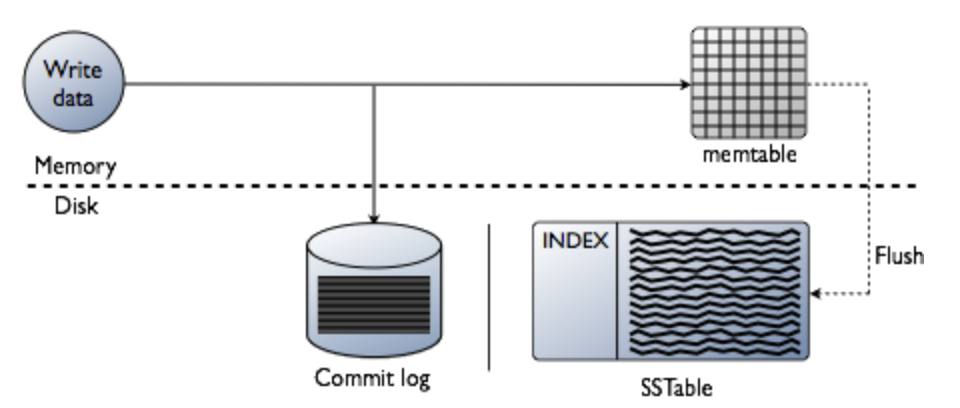
\includegraphics[width=0.8\textwidth]{assets/casandra.png}
    \caption{Схема записи в Casandra}
    \label{fig:mesh1}
\end{figure}

\paragraph{PostreSQL + Patroni}
Patroni — это Python-приложение для создания высокодоступных PostgreSQL кластеров на основе потоковой репликации. С его помощью можно преобразовать систему из ведущего и ведомых узлов (primary — replica) в высокодоступный кластер с поддержкой автоматического контролируемого (switchover) и аварийного (failover) переключения. Patroni позволяет легко добавлять новые реплики в существующий кластер, поддерживает динамическое изменение конфигурации PostgreSQL одновременно на всех узлах кластера и множество других возможностей, таких как синхронная репликация, настраиваемые действия при переключении узлов, REST API, возможность запуска пользовательских команд для создания реплики вместо pg_basebackup, взаимодействие с Kubernetes и т.д.(\autocite{Klyukin}) \\
Опишем, как используется Patroni. Сама по себе потоковая репликация не является достаточным средством обеспечения высокой доступности. Потому что нет никакого встроенного решения, которое бы позволило перевести standby в режим нового мастера, если что-то произошло со старым мастером. Рассмотрим на примере (\autocite{Aristov}).\\
Возьмем кластер из двух нод, и, допустим, у нас есть программа, запущенная на standby-сервере, мониторящая, жив ли основной сервер, и при его падении повышающая реплику до основного сервера:

\begin{figure}[h]
    \centering
    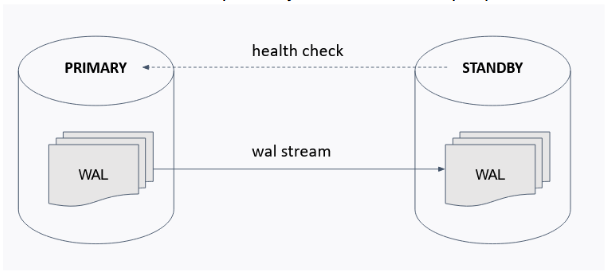
\includegraphics[width=0.8\textwidth]{assets/Patroni1.png}
    \caption{Кластер из двух нод}
    \label{fig:mesh1}
\end{figure}

Вроде всё хорошо, но что произойдёт, если у нас просто случится обрыв сетевого подключения между серверами?

\begin{figure}[h]
    \centering
    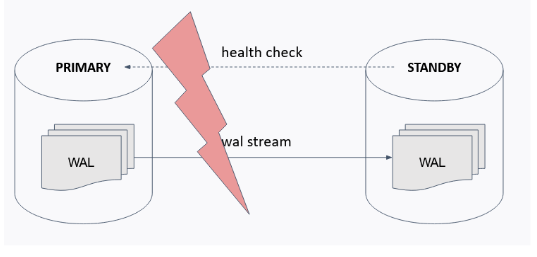
\includegraphics[width=0.8\textwidth]{assets/Patroni2.png}
    \caption{Кластер из двух нод}
    \label{fig:mesh1}
\end{figure}

Правильно! Получим два независимых основных кластера, каждый из них будет принимать запросы на запись, и мы получим такую ситуацию:

\begin{figure}[h]
    \centering
    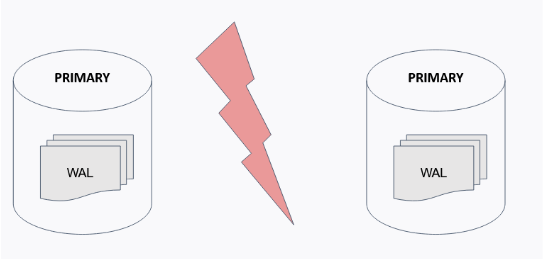
\includegraphics[width=0.8\textwidth]{assets/Patroni3.png}
    \caption{Разрыв соединения в кластере из двух нод}
    \label{fig:mesh1}
\end{figure}

Она называется splitbrain. Это очень плохая ситуация, и в дальнейшем объединить изменённые данные с двух независимых серверов без потерь практически нереально.
Казалось бы, есть простое решение - добавить стороннего наблюдателя.
Что же может пойти не так в данной конфигурации:

\begin{figure}[h]
    \centering
    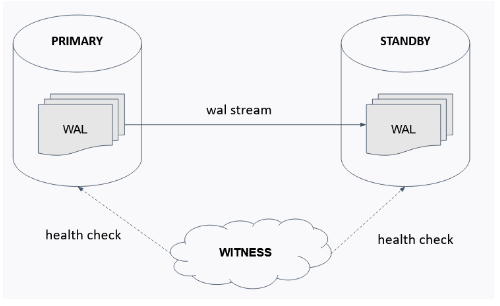
\includegraphics[width=0.8\textwidth]{assets/Patroni4.png}
    \caption{Кластер из двух нод со сторонним наблюдателем}
    \label{fig:mesh1}
\end{figure}

В такой конфигурации могут возникнуть две проблемы: во-первых, может умереть наблюдатель и мониторить станет некому, во-вторых, может оборваться соединение с основной нодой и опять мы получаем splitbrain. 
И Patroni предлагает решение данной проблемы - это использование отказоустойчивого кластера для наблюдателя, в котором мы будем хранить статус активного сервера. То есть основной будет активно ходить и поддерживать статус основного, а остальные будут опрашивать жив ли основной сервер. При потере с ним соединения через некоторое время произойдут выборы и вторичный сервер станет основным и будет активно поддерживать свой статус в этом отказоустойчивом наблюдателе. При этом изначальный основной сервер при недоступности кластера наблюдения перейдёт в статус “только чтение".

\begin{figure}[h]
    \centering
    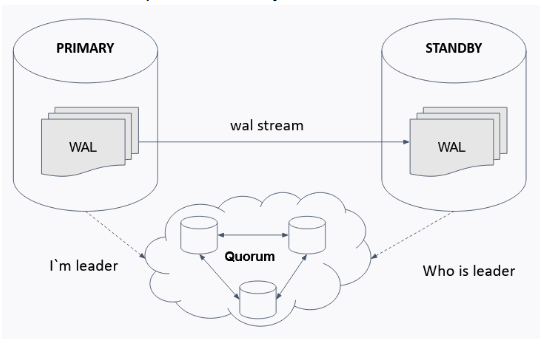
\includegraphics[width=0.8\textwidth]{assets/Patroni5.png}
    \caption{Решение, используемое в Patroni}
    \label{fig:mesh1}
\end{figure}

Quorum позволяет нам решать сложные задачи разрешения партицирования сети. Когда какой-то сегмент сети недоступен, то несколько других сегментов могут принимать решения. А изолированный сегмент в этом случае должен остановить старого мастера. 